\documentclass{standalone}
\usepackage{tikz}
\usetikzlibrary{arrows.meta}

\begin{document}
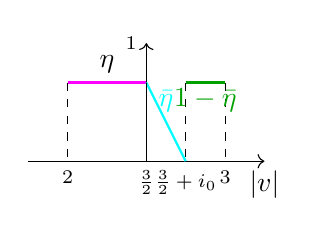
\begin{tikzpicture}[scale=1.0]

% Colors
\definecolor{myMagenta}{HTML}{FF00FF}
\definecolor{myCyan}{HTML}{00FFFF}
\definecolor{myGreen}{HTML}{00A000}

% Axes
\draw[->] (-1.5,0) -- (1.5,0) node[below] {$|v|$};
\draw[->] (0,0) -- (0,1.5) node[left] {\scriptsize $1$};

% Lines
\draw[myMagenta,thick] (-1,1) -- (0,1);
\draw[myCyan,thick] (0,1) -- (0.5,0);
\draw[myGreen,thick] (0.5,1) -- (1,1);

% Dotted Lines and Nodes
\draw[dashed] (-1,1) -- (-1,0) node[below] {\scriptsize $2$};
\draw[dashed] (0,1) -- (0,0) node[below] {\scriptsize $\frac{3}{2}$};
\draw[dashed] (0.5,1) -- (0.5,0) node[below] {\scriptsize $\frac{3}{2}+i_0$};
\draw[dashed] (1,1) -- (1,0) node[below] {\scriptsize $3$};

% Annotations
\node[above] at (-0.5,1) {\mymagenta{$\eta$}};
\node[above] at (0.25,0.5) {\textcolor{myCyan}{$\bar{\eta}$}};
\node[above] at (0.75,0.5) {\textcolor{myGreen}{$1-\bar{\eta}$}};

\end{tikzpicture}
\end{document}